%-------------------------------------------------------------------------------
% RESULTS
%-------------------------------------------------------------------------------

\section{Results} \label{sec:res}

% \begin{table}[h!]
%   \caption{List of bifurcations encountered and the critical $\Rey$ at which they
%     occur}
%   \label{tab:bif_points}
% \begin{tabular}{l c}
% Bifurcation & $\Rey$\\
% \hline
% $P_1$, first pitchfork of the base flow & \\
% $P_2$, second pitchfork of the base flow & \\
% $SN$, saddle-node bifurcation of the asymmetric steady solution&  \\
% $H$, Hopf bifurcation of the asymmetric steady solution&  \\
% \end{tabular}
% \end{table}
%
%
% \begin{table}[h!]
%   \caption{Critical Reynolds numbers of the two
%     pitchfork bifurcations of the symmetric base flow, $\Rey_c^{P_1}$
%     and $\Rey_c^{P_2}$, and of the saddle-node and Hopf bifurcations
%     corresponding to the asymmetric steady solution, $\Rey_c^{H}$ and
%     $\Rey_c^{SN}$, respectively. For the Hopf bifurcation, the imaginary part
%     $\omega_c^{H}$ corresponding to the crossing eigenvalue has also been
%     included.}
%   \label{tab:re_crit}
% \begin{tabular}{crrrrrr}
% $M$ & $\Rey_c^{P_1}$ & $\Rey_c^{P_2}$ & $\Rey_c^{H}$ &  $\omega_c^{H}$ & $\Rey_c^{SN}$  \\
% \hline
% $48$ &  & &          &          &   \\
% $64$ &  & &          &          &   \\
% $96$ &  & &          &          &   \\
% \end{tabular}
% \end{table}

% \begin{figure}[h!]
%   \begin{center}
%   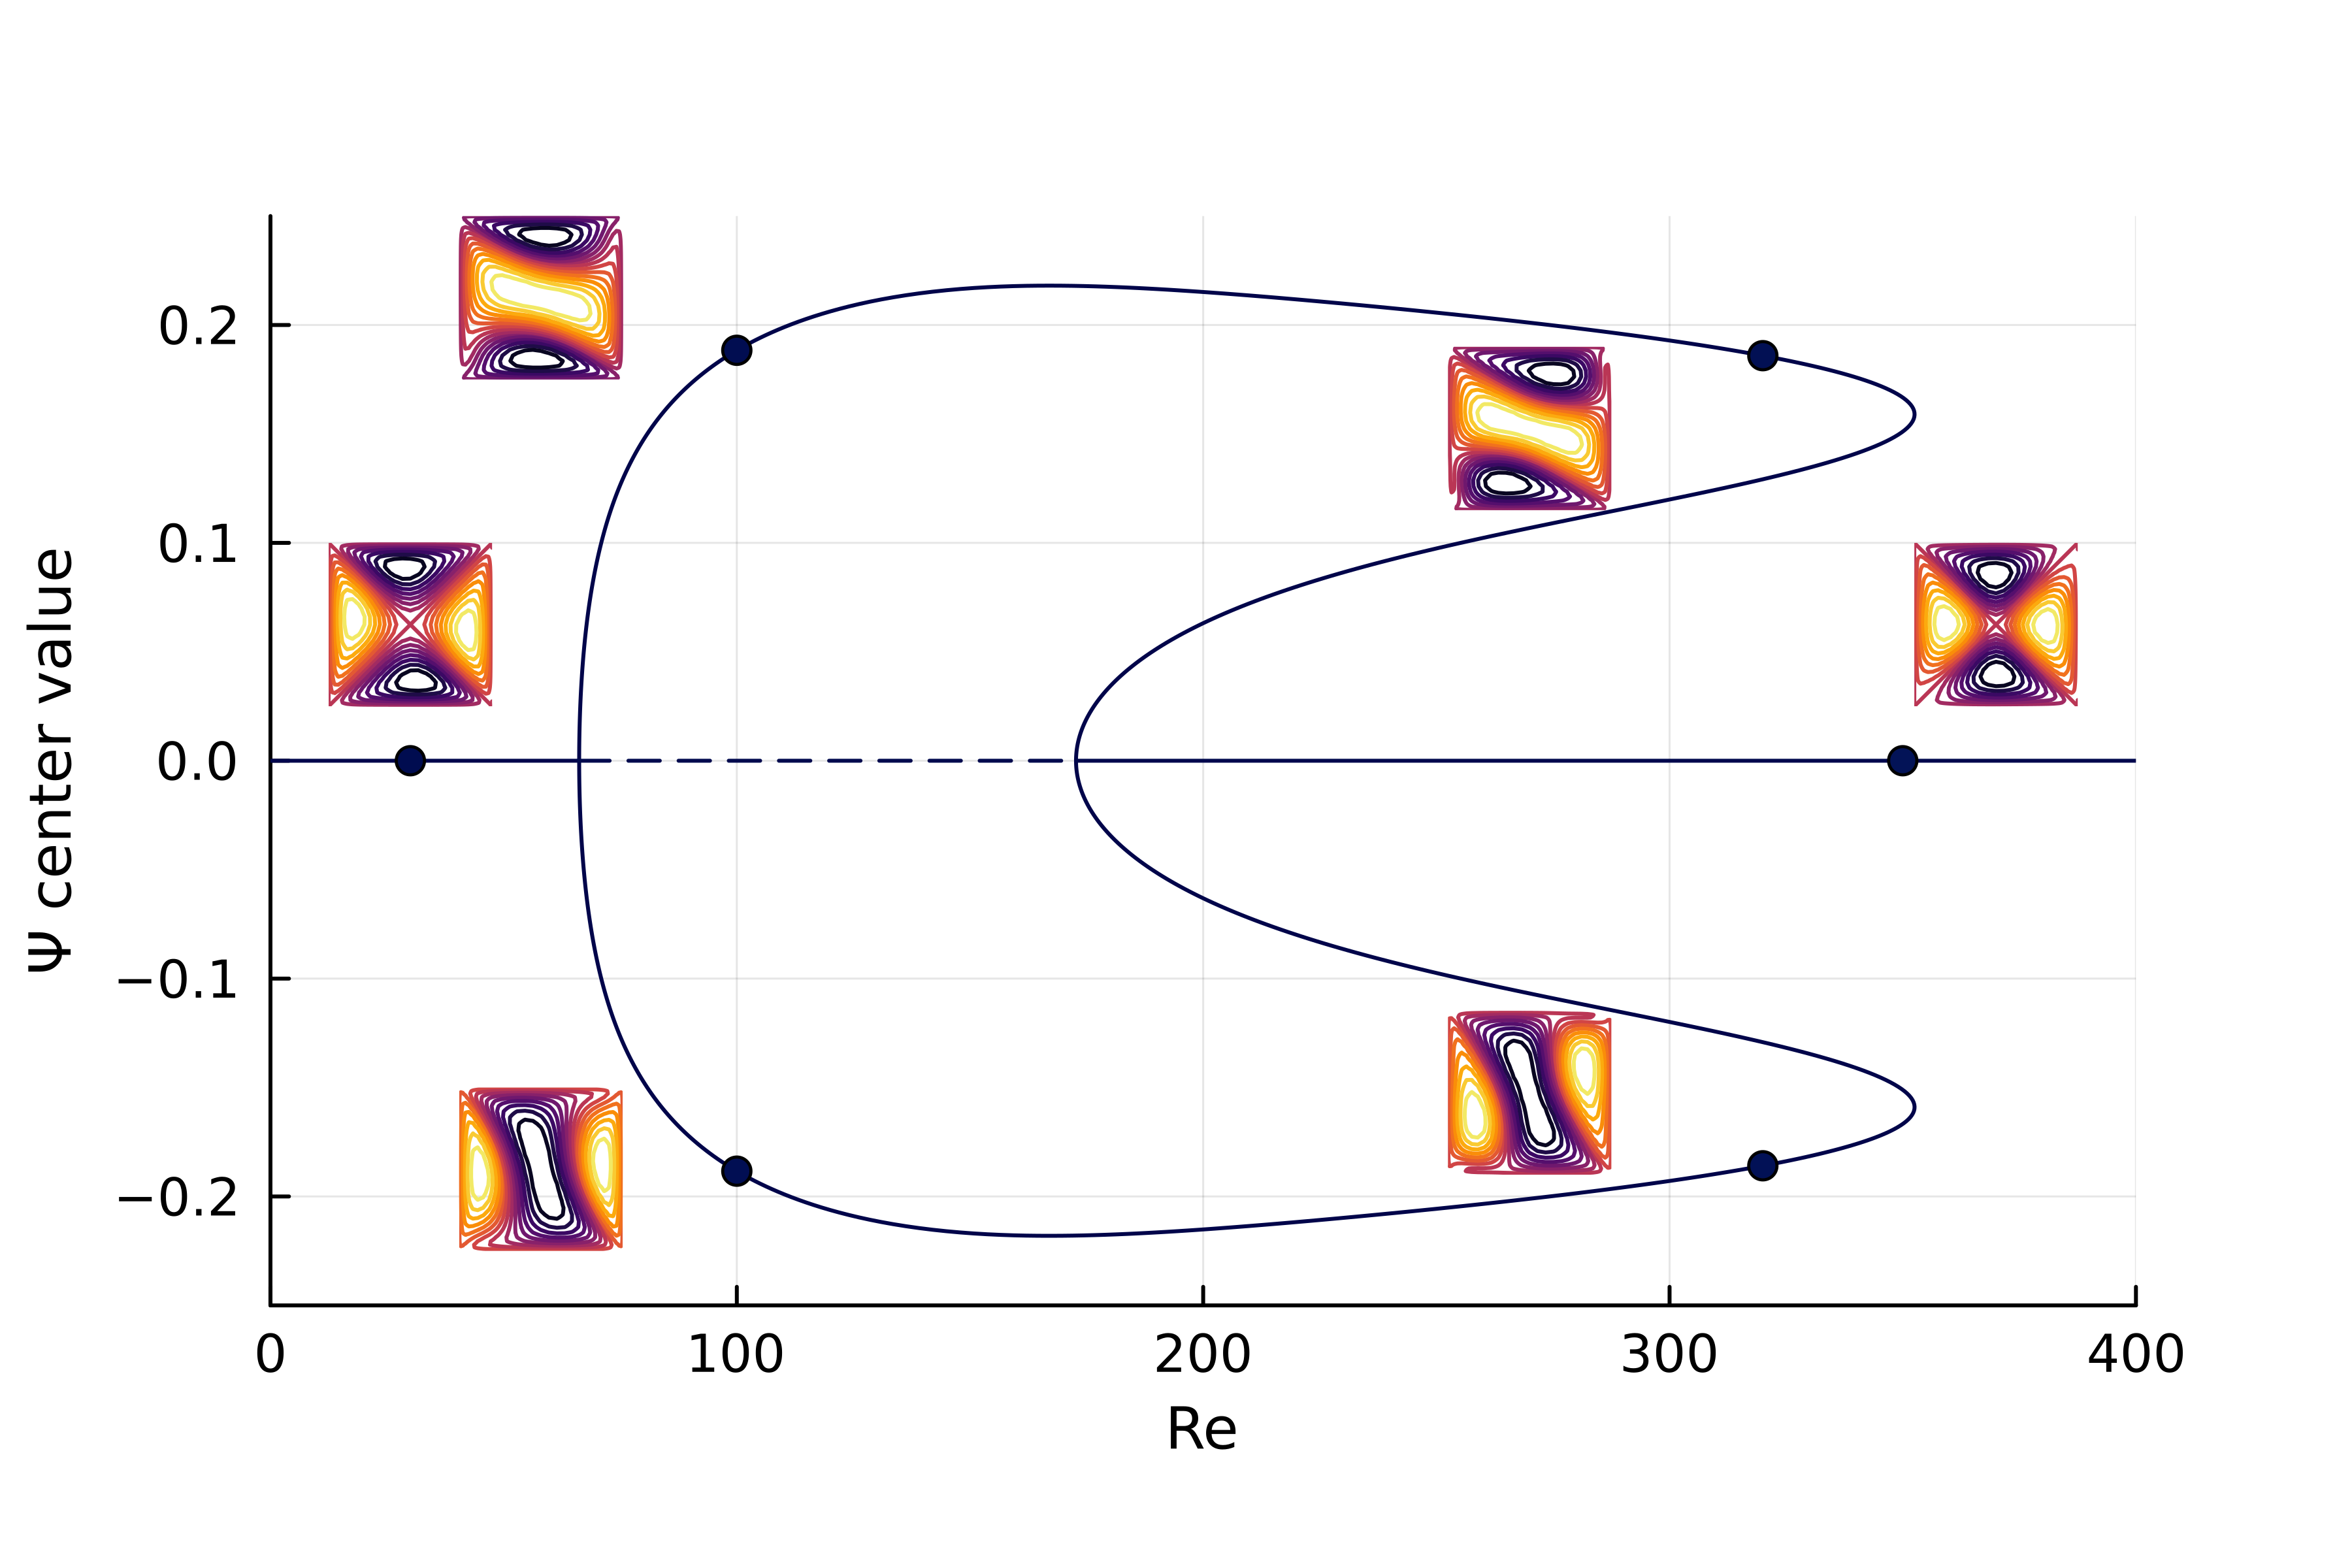
\includegraphics[width=0.8\textwidth]{figs/32x32_bif_diagram.png}
%   \end{center}
%   \label{fig:bif_diag}
%   \caption{Bifurcation diagram for the regularized version of the four-sided
%     cavity flow, calculated through the developed Julia package} 
% \end{figure}
